% Three content pages follow the unchanged separate reference-style cover.
\section{Sunflower detection using scale-space extrema}
\smallnote{\textbf{Repository:} \url{https://github.com/ahesh-dilhan/en3160-assignment-02}}
The supplied image is read with \texttt{cv.IMREAD\_REDUCED\_COLOR\_4}, giving
$360\times360$ pixels. Dark central disks are detected using darkness
$D=1-I_{\rm gray}/255$ and scale-normalized LoG response
$L=-\sigma^2\nabla^2(G_\sigma*D)$. Positive spatial/scale maxima indicate dark
blobs; their ideal-disk radius estimate is $r=\sqrt{2}\sigma$.
\begin{lstlisting}
L = np.stack([-s*s*gaussian_laplace(D, s) for s in sigmas])
peaks = (L == maximum_filter(L, size=(3, 3, 3))) & (L >= 0.12)
\end{lstlisting}
\textbf{Parameters.} Use 36 geometric scales, $\sigma\in[1.5,16]$ pixels,
excluding end-scale maxima; threshold 0.12; permitted overlap 35\% of the smaller
disk area. Yellow-petal support must cover 50\% of the annulus $[r,2.2r]$ with
angular coverage. A Hessian curvature ratio $\geq0.5$ rejects elongated gaps.
No Hough-circle detector is used.

\begin{minipage}[t]{0.53\linewidth}\vspace{0pt}
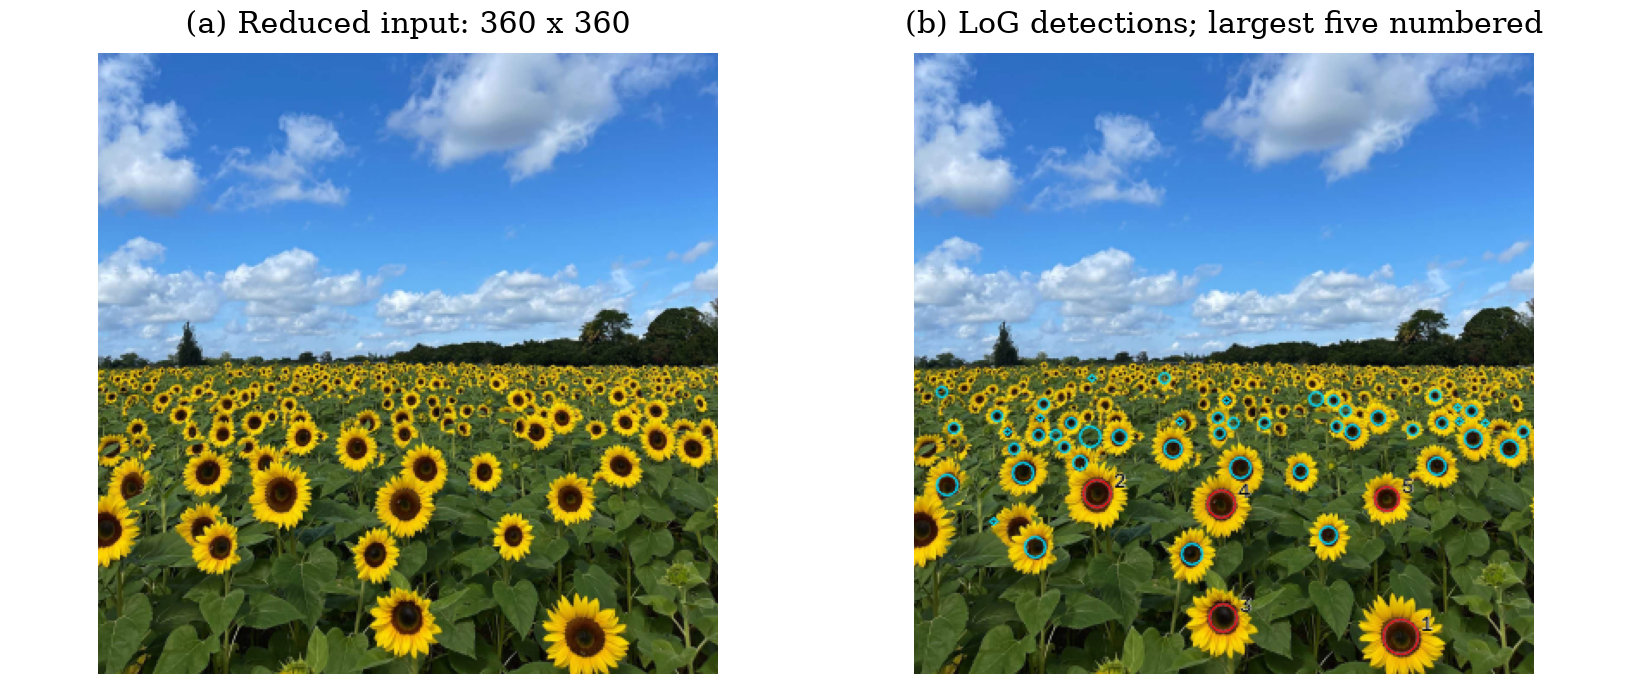
\includegraphics[width=\linewidth]{figures/sunflowers.png}
\figcaption{Input and \BlobCount{} candidates. The largest five disks are numbered.}
\end{minipage}\hfill
\begin{minipage}[t]{0.44\linewidth}\vspace{7pt}\centering\footnotesize
\setlength{\tabcolsep}{3pt}
\begin{tabular}{rrrrrr}
\toprule Rank & $x$ & $y$ & $\sigma$ & $r$ & Response\\\midrule
\BlobRows\bottomrule
\end{tabular}
\par\vspace{3pt}Coordinates and radii are in reduced-image pixels.
\end{minipage}

\textbf{Interpretation.} The largest disk is at $(282,338)$, $r=10.05$ pixels.
The origin is top-left; multiply coordinates and radii by four for original-image
units. The prior suppresses foliage but misses distant, tilted or occluded
flowers. These are candidates, not a verified count; radii describe central
disks rather than complete blossoms.

\section{Custom RANSAC: line followed by circle}
\textbf{Data.} Listing 1 is reproduced with seed 0: 50 circle points with centre
$(2,3)$, radius 10 and radial-noise standard deviation 0.625, plus 50 points from
$y=-x+2$ with vertical-noise standard deviation 1. Both loops are hand-written:
two distinct points define a line hypothesis; three non-collinear points define
a circle. Degenerate samples are rejected. Each model uses 2,000 trials; the
sequence starts with RNG seed 100.

\textbf{Residuals and consensus.} Represent the line by $ax+by=d$ with
$a^2+b^2=1$, $d\geq0$. The errors are
\[
e_\ell(\mathbf p)=|ap_x+bp_y-d|,\qquad
e_c(\mathbf p)=\bigl|\|\mathbf p-\mathbf c\|_2-r\bigr|.
\]
Both thresholds are 1.5: approximately 2.12 normal-noise standard deviations
for the true line and 2.4 for the circle. Require at least 35 line inliers,
remove that consensus, and require at least 25 circle inliers from the remainder.
TLS refines the line; L-BFGS-B minimizes mean squared radial error with $r>0$.
Membership is updated after refinement; winning samples and unrefined models
are retained separately.
\begin{lstlisting}
line = ransac(X, "line", rng, threshold=1.5, minimum_consensus=35)
remaining = np.flatnonzero(~line.inliers)
circle = ransac(X[remaining], "circle", rng,
                threshold=1.5, minimum_consensus=25)
\end{lstlisting}
For $p=0.99$, $w=0.5$ and sample size $s$,
$N=\lceil\log(1-p)/\log(1-w^s)\rceil$ gives 17 line or 35 circle trials.
The larger fixed budget accommodates contamination and reduced inlier fractions;
it does not guarantee success.

\vspace{-5pt}
\begin{center}\small
\begin{tabular}{llrr}
\toprule Model & Refined parameters & Inliers & Inlier RMSE\\\midrule
\FitRows\bottomrule
\end{tabular}\end{center}
\textbf{Circle first.} Seed 0 also succeeds: centre $(1.943,3.008)$, radius
9.930. For data seeds 0--19, circle recovery occurs in 20/20 line-first and
19/20 circle-first runs, defining recovery as centre and radius errors below 2.
A large-radius circle can approximate a line and steal its consensus, although
circle-first need not fail. Line-first can remove genuine circle points near
intersections, explaining its 54-point consensus. Refinement is local, not a
proof of global optimality.


\newpage
\textbf{RANSAC results and fitting-order comparison}
\begin{center}
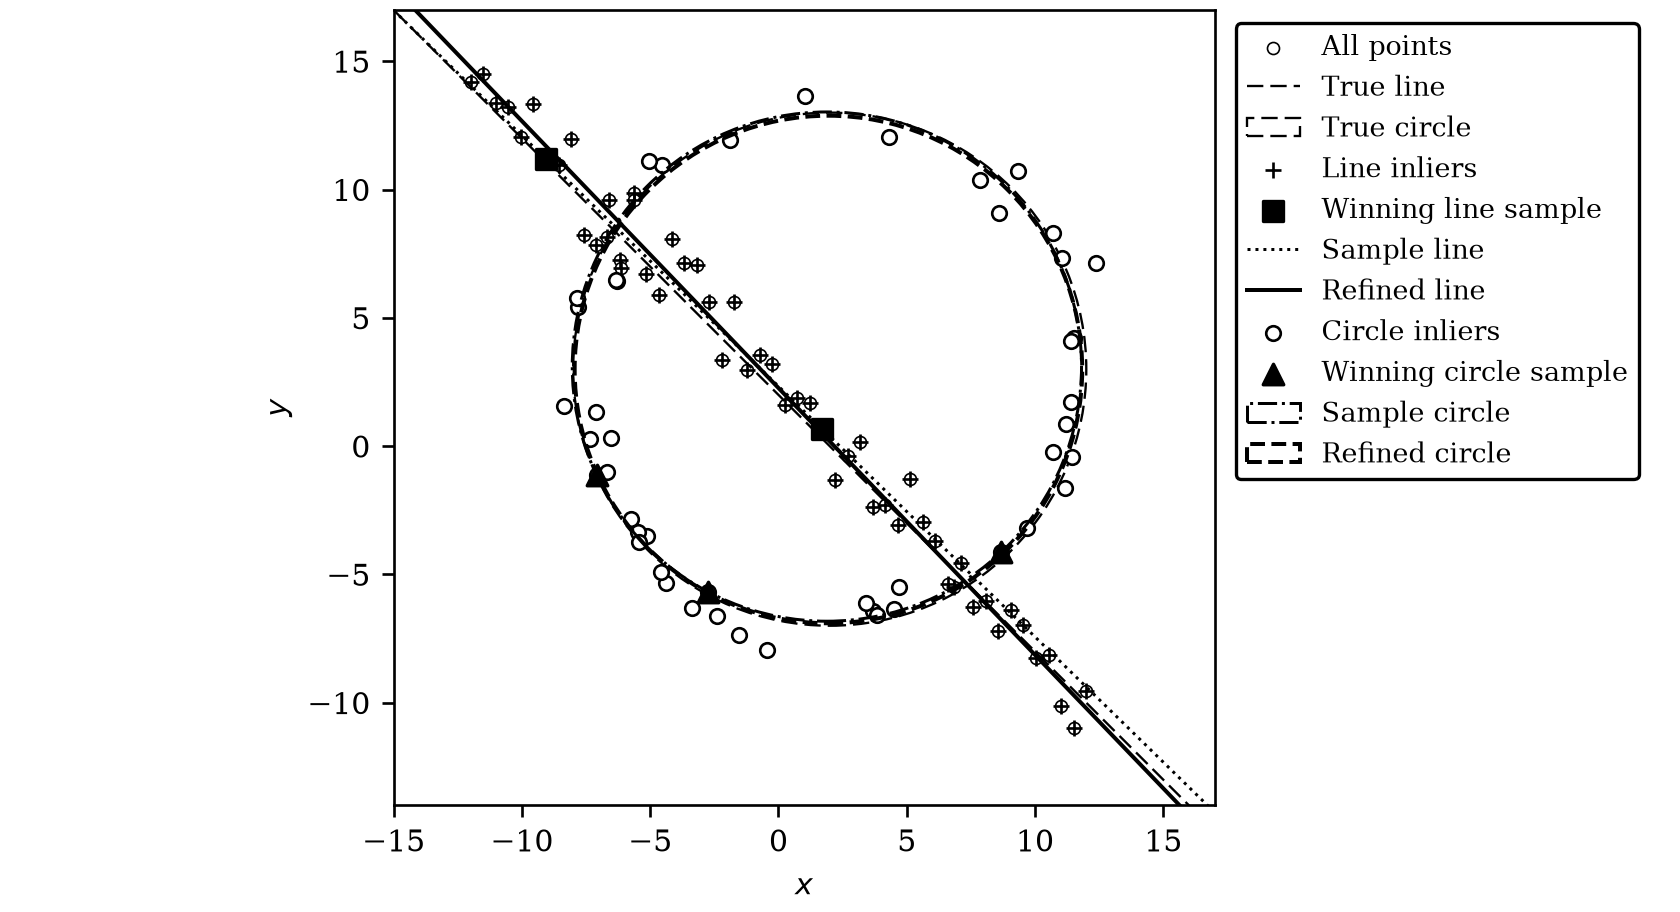
\includegraphics[width=0.85\linewidth]{figures/ransac.png}
\figcaption{All points, winning samples, sample hypotheses, refined models and
their line/circle consensus sets, shown together.}
\end{center}
\section{Planar homography and image compositing}
Two architectural photographs are paired with original graphics: an open-studio
banner on a flat facade band (oblique view) and a community-garden notice on a
garage door (nearly frontal). Both notices are fictional. Four destination
corners are ordered TL, TR, BR, BL. They were selected visually, not recorded
mouse clicks; \texttt{select\_corners.py} provides four-click selection.

\begin{center}
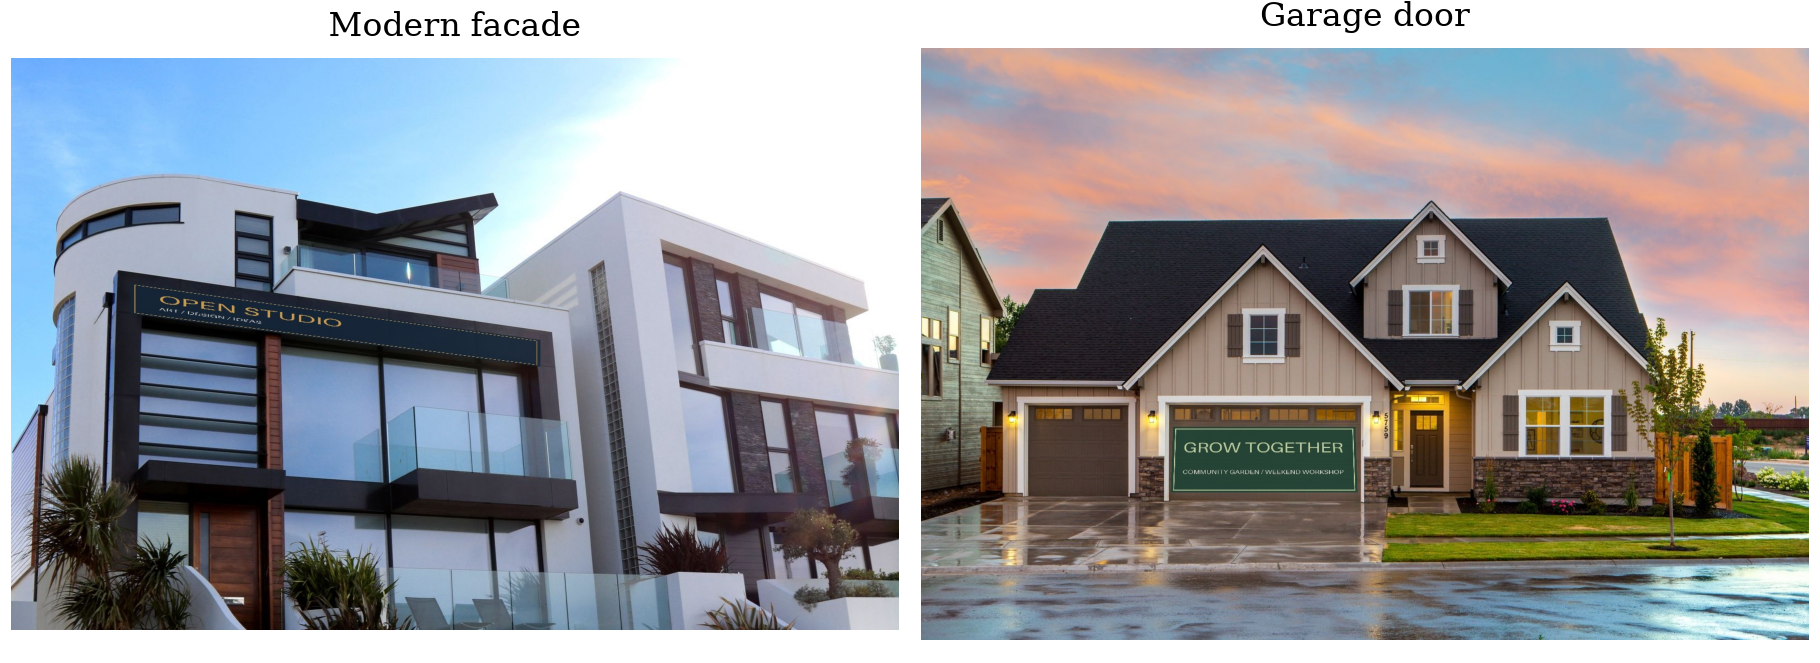
\includegraphics[width=0.94\linewidth]{figures/composites_compact.png}
\figcaption{Composited results for the two chosen image pairs, retaining original
colours. Inputs and original overlay graphics are available in the repository.}
\end{center}
\vspace{-5pt}
The four source/destination pairs define $\mathbf x'\sim H\mathbf x$, mapping
overlay to background. Warp the graphic and an all-one coverage mask with the
same bilinear interpolation. With premultiplied warped colour $W$ and coverage
$M$, $C=B(1-\alpha M)+\alpha W$; black graphic pixels remain valid content.
\begin{lstlisting}
H = cv.getPerspectiveTransform(source_corners, destination_corners)
result = background*(1-alpha*M[..., None]) + alpha*W
\end{lstlisting}
\begin{center}\footnotesize
\begin{tabular}{llr}
\toprule Pair & Destination corners (pixels) & $\alpha$\\\midrule
\CornerRows\bottomrule
\end{tabular}\end{center}
Corner reprojection error is below 0.001 pixels, confirming correspondence rather
than independent accuracy: the same points define $H$. Alpha blending retains
texture but does not model physical illumination, shadows, reflections or
occlusion. The facade placement is more distorted than the garage placement.

\smallnote{\textbf{Image credits.} Expect Best,
\href{https://www.pexels.com/photo/modern-building-against-sky-323780/}{Pexels 323780};
Binyamin Mellish,
\href{https://www.pexels.com/photo/brown-and-gray-painted-house-in-front-of-road-1396122/}{Pexels 1396122}.
Downloaded at width 1600; original graphics added.
\href{https://www.pexels.com/license/}{Pexels license}; full attribution in the repository.}
